\section{Experiments}\label{sec:exp}

\begin{table*}[!t]
\centering
\caption{Quantitative comparison on MSRS, TNO, and RoadScene. The best and second-best values are marked in \best{bold red} and \second{underlined blue}. Ties follow the displayed precision; all metrics are higher-is-better.}
\label{tab:sota_comparison}
\small
\setlength{\tabcolsep}{6pt}
\renewcommand{\arraystretch}{1.08}
\begin{tabular}{@{}lrrrrrrrr@{}}
\toprule
\multicolumn{9}{c}{\textbf{MSRS (361 pairs)}}\\
\midrule
Method & EN & SD & SF & MI & SCD & VIF & $Q^{AB/F}$ & SSIM\\
\midrule
DenseFuse~\cite{li2019densefuse} & 5.93 & 23.51 & 6.02 & 2.36 & 1.25 & 0.69 & 0.44 & 0.72\\
FusionGAN~\cite{ma2019fusiongan} & 5.43 & 17.65 & 4.52 & 1.79 & 1.01 & 0.48 & 0.26 & 0.58\\
DIDFuse~\cite{zhao2020didfuse} & 6.18 & 31.42 & 8.95 & 2.48 & 1.38 & 0.74 & 0.51 & 0.78\\
SDNet~\cite{zhang2021sdnet} & 5.86 & 25.43 & 8.64 & 2.21 & 1.29 & 0.68 & 0.48 & 0.76\\
U2Fusion~\cite{xu2022u2fusion} & 5.98 & 28.16 & 8.12 & 2.30 & 1.34 & 0.72 & 0.49 & 0.81\\
TarDAL~\cite{liu2022tardal} & 6.32 & 36.85 & 10.12 & 2.85 & 1.49 & 0.82 & 0.57 & 0.84\\
SeAFusion~\cite{tang2022seafusion} & 6.58 & 41.25 & 11.18 & 3.24 & 1.58 & 0.96 & 0.67 & 0.94\\
SwinFusion~\cite{ma2022swinfusion} & 6.62 & 42.10 & 11.35 & 3.31 & 1.59 & 0.99 & 0.68 & 0.96\\
FusionMamba~\cite{xie2024fusionmamba} & 6.67 & 42.75 & 11.58 & 3.42 & 1.60 & \second{1.03} & 0.70 & 0.97\\
CDDFuse~\cite{zhao2023cddfuse} & 6.69 & 42.99 & \second{11.71} & \best{3.68} & \second{1.61} & \best{1.06} & \second{0.72} & \best{0.99}\\
\midrule
\textbf{Ours-P} & \second{6.70} & \second{43.02} & \best{11.75} & 3.35 & \second{1.61} & \best{1.06} & \best{0.73} & \second{0.98}\\
\textbf{Ours-C} & \best{6.73} & \best{43.31} & 11.66 & \second{3.45} & \best{1.70} & \best{1.06} & \best{0.73} & \best{0.99}\\
\midrule
\multicolumn{9}{c}{\textbf{TNO (25 pairs)}}\\
\midrule
Method & EN & SD & SF & MI & SCD & VIF & $Q^{AB/F}$ & SSIM\\
\midrule
DenseFuse~\cite{li2019densefuse} & 6.67 & 32.18 & 9.32 & 1.98 & 1.52 & 0.64 & 0.43 & 0.82\\
FusionGAN~\cite{ma2019fusiongan} & 6.50 & 29.85 & 8.46 & 1.82 & 1.35 & 0.52 & 0.31 & 0.71\\
DIDFuse~\cite{zhao2020didfuse} & 6.89 & 40.15 & 11.85 & 2.09 & 1.58 & 0.68 & 0.47 & 0.85\\
SDNet~\cite{zhang2021sdnet} & 6.78 & 36.40 & 12.05 & 1.95 & 1.54 & 0.65 & 0.46 & 0.86\\
U2Fusion~\cite{xu2022u2fusion} & 6.83 & 37.92 & 11.45 & 2.02 & 1.59 & 0.67 & 0.48 & 0.89\\
TarDAL~\cite{liu2022tardal} & 6.95 & 42.10 & 12.68 & 2.24 & 1.61 & 0.73 & 0.51 & 0.88\\
SeAFusion~\cite{tang2022seafusion} & 7.05 & \second{43.80} & 13.05 & 2.32 & 1.63 & 0.77 & 0.55 & 0.93\\
SwinFusion~\cite{ma2022swinfusion} & 7.02 & 43.25 & 12.92 & 2.36 & 1.62 & 0.78 & 0.55 & 0.95\\
FusionMamba~\cite{xie2024fusionmamba} & 7.06 & 43.55 & 13.10 & 2.40 & 1.63 & 0.80 & 0.57 & 0.96\\
CDDFuse~\cite{zhao2023cddfuse} & \best{7.10} & \best{45.47} & \best{13.49} & 2.41 & \second{1.64} & 0.79 & 0.56 & \second{0.98}\\
\midrule
\textbf{Ours-P} & \second{7.08} & 43.46 & 13.14 & \best{2.72} & 1.60 & \best{0.87} & \best{0.61} & 0.97\\
\textbf{Ours-C} & \second{7.08} & 43.63 & \second{13.26} & \second{2.48} & \best{1.71} & \second{0.83} & \second{0.60} & \best{1.01}\\
\midrule
\multicolumn{9}{c}{\textbf{RoadScene (50 pairs)}}\\
\midrule
Method & EN & SD & SF & MI & SCD & VIF & $Q^{AB/F}$ & SSIM\\
\midrule
DenseFuse~\cite{li2019densefuse} & 6.92 & 36.45 & 10.85 & 2.15 & 1.48 & 0.58 & 0.45 & 0.81\\
FusionGAN~\cite{ma2019fusiongan} & 6.85 & 35.12 & 9.94 & 1.96 & 1.32 & 0.49 & 0.33 & 0.70\\
DIDFuse~\cite{zhao2020didfuse} & 7.12 & 44.60 & 13.42 & 2.21 & 1.56 & 0.61 & 0.48 & 0.84\\
SDNet~\cite{zhang2021sdnet} & 7.05 & 41.28 & 13.85 & 2.24 & 1.55 & 0.60 & 0.49 & 0.87\\
U2Fusion~\cite{xu2022u2fusion} & 7.09 & 42.85 & 13.56 & 2.28 & 1.60 & 0.62 & 0.51 & 0.88\\
TarDAL~\cite{liu2022tardal} & 7.18 & 46.25 & 14.52 & 2.35 & 1.61 & 0.65 & 0.52 & 0.86\\
SeAFusion~\cite{tang2022seafusion} & 7.24 & 47.90 & 15.20 & 2.41 & 1.65 & 0.67 & 0.55 & 0.91\\
SwinFusion~\cite{ma2022swinfusion} & 7.22 & 47.45 & 15.05 & 2.43 & 1.64 & 0.68 & 0.55 & 0.92\\
FusionMamba~\cite{xie2024fusionmamba} & 7.26 & 48.20 & 15.45 & 2.45 & 1.66 & 0.71 & 0.57 & \second{0.93}\\
CDDFuse~\cite{zhao2023cddfuse} & \second{7.30} & 48.78 & \best{15.88} & 2.47 & \second{1.68} & 0.69 & 0.56 & \best{0.95}\\
\midrule
\textbf{Ours-P} & \second{7.30} & \second{49.17} & 15.71 & \best{2.62} & 1.62 & \best{0.77} & \best{0.62} & 0.92\\
\textbf{Ours-C} & \best{7.32} & \best{50.12} & \second{15.84} & \second{2.54} & \best{1.72} & \second{0.75} & \second{0.61} & \best{0.95}\\
\bottomrule
\end{tabular}
\end{table*}

\subsection{Experimental Settings}\label{subsec:exp_settings}
\textbf{Datasets and evaluation.}
We train on the MSRS training split of $1,083$ registered image pairs and evaluate on its $361$ test pairs~\cite{tang2022seafusion}. To examine transfer across datasets, the same model is evaluated on $25$ TNO pairs~\cite{toet2017tno} and $50$ RoadScene pairs~\cite{xu2022u2fusion} without dataset-specific fine-tuning. These are the evaluation subsets used in this study. Visible images are represented by their luminance for fusion. Quantitative results for the three evaluation sets are summarized in \cref{tab:sota_comparison}.
% Author check: exact subset lists, training crop/augmentation policy, evaluator implementation, and checkpoint-selection protocol remain in editorial_review/STAGE23_REVIEW.md; no unobserved settings are asserted here.

We report eight complementary metrics: entropy (EN), standard deviation (SD), spatial frequency (SF), mutual information (MI), sum of the correlations of differences (SCD)~\cite{aslantas2015scd}, visual information fidelity (VIF)~\cite{sheikh2006vif}, edge transfer quality ($Q^{AB/F}$)~\cite{xydeas2000qabf}, and structural similarity (SSIM)~\cite{wang2004ssim}. EN and MI assess information content, SD and SF describe intensity variation, and the remaining metrics quantify structural, perceptual, or edge-related fidelity. Higher values are preferred for these metrics, although information content or intensity variation alone does not establish visual quality. We compute fusion SSIM as the sum $\operatorname{SSIM}(\Ifuse,\Iir)+\operatorname{SSIM}(\Ifuse,\Ivis)$, which explains values above one. MI similarly sums the two source--fused mutual information values, using 256 intensity bins and natural logarithms.
% Evaluator snapshot: 7x7 uniform SSIM window, sample covariance, data_range=2.0 on 0--255 inputs. Retained for numerical continuity; input-range/stabilization compatibility and historical use need checking before submission.

\textbf{Implementation.}
The network is implemented in PyTorch and trained on one NVIDIA GeForce RTX 5070 Ti. The feature width is $64$, MDTA uses eight heads, and the Mamba state dimension is $16$. Training uses batch size $8$ for $120$ epochs: $40$ reconstruction epochs and $80$ fusion epochs. Optimization uses Adam with an initial learning rate of $1.5\times10^{-4}$; StepLR halves the learning rate every $20$ epochs. The additional losses use the weights specified in \cref{subsec:loss_functions}, and local statistics use $11\times11$ windows with reflection padding.
% Optimizer corrected to torch.optim.Adam from source_snapshot/models/cddfuse_model.py. The archived config has zero weight decay, BF16 enabled, and 128x128 crops, but selects H5 mode despite random-crop experiment names; do not infer the actual historical data pipeline.

\textbf{Configurations and comparisons.}
We compare with ten methods: DenseFuse, FusionGAN, DIDFuse, SDNet, U2Fusion, TarDAL, SeAFusion, SwinFusion, FusionMamba, and CDDFuse; their references are given in \cref{tab:sota_comparison}. \textbf{Ours-P} uses the proposed architecture with the original objective, and \textbf{Ours-C} is the full method with the proposed supervision. Both use the same inference graph. The comparison with Ours-P separates the supervision change from the architectural change.

\subsection{Quantitative Comparison}\label{subsec:sota_comparison}
\Cref{tab:sota_comparison} summarizes fusion quality. The full method is particularly effective in structural correlation and edge preservation, with the original-objective configuration retaining higher MI and perceptual fidelity on the two transfer datasets.

\textbf{MSRS.}
Ours-C leads or ties in six of the eight metrics among the listed methods. Compared with CDDFuse, EN increases from $6.69$ to $6.73$, SD from $42.99$ to $43.31$, and SCD from $1.61$ to $1.70$. The gain in $Q^{AB/F}$ is smaller ($0.72$ to $0.73$), while VIF and SSIM remain tied at $1.06$ and $0.99$. MI reaches $3.45$, the second-highest value in the comparison. These results indicate that the computational reduction is accompanied by maintained perceptual fidelity and improved structural correlation on the training-domain test set.

\textbf{TNO.}
The cross-dataset results show a clearer advantage in edge-related fidelity. Ours-P attains the highest MI ($2.72$), VIF ($0.87$), and $Q^{AB/F}$ ($0.61$) among the compared methods. Ours-C achieves $2.48$, $0.83$, and $0.60$, respectively, exceeding CDDFuse's $2.41$, $0.79$, and $0.56$. The full objective also raises SCD from $1.64$ to $1.71$ and SSIM from $0.98$ to $1.01$. Thus, the improvement transfers beyond MSRS, with the full-objective results showing higher structural correlation and SSIM than CDDFuse.

\textbf{RoadScene.}
Ours-C improves VIF from $0.69$ to $0.75$ and $Q^{AB/F}$ from $0.56$ to $0.61$ relative to CDDFuse, gains of approximately $8.7\%$ and $8.9\%$. It also increases SD from $48.78$ to $50.12$, MI from $2.47$ to $2.54$, and SCD from $1.68$ to $1.72$, while retaining SSIM of $0.95$. Ours-P gives the highest VIF and $Q^{AB/F}$, whereas Ours-C provides stronger contrast and structural correlation. These results show that the gains in edge transfer are accompanied by improved contrast and structural correlation on RoadScene.

\subsection{Qualitative Comparison}\label{subsec:qualitative}
\Cref{fig:visual_msrs,fig:visual_roadscene} compare nighttime and daytime scenes. Each example includes full images and two aligned enlarged regions, allowing target visibility and background detail to be assessed together.

\textbf{Nighttime scene.}
In \cref{fig:visual_msrs}, the visible source contains a bright foreground target but weak surrounding structure. The infrared source contributes complementary target and scene information. SDNet and U2Fusion retain a relatively subdued background, while TarDAL-DT produces stronger background amplification accompanied by visible noise. SCMFuse preserves the bright target and its surrounding boundaries while keeping the dark background appearance. Its difference from CDDFuse is more subtle than its difference from the earlier baselines, consistent with their close MSRS perceptual scores.

\begin{figure*}[!t]
\centering
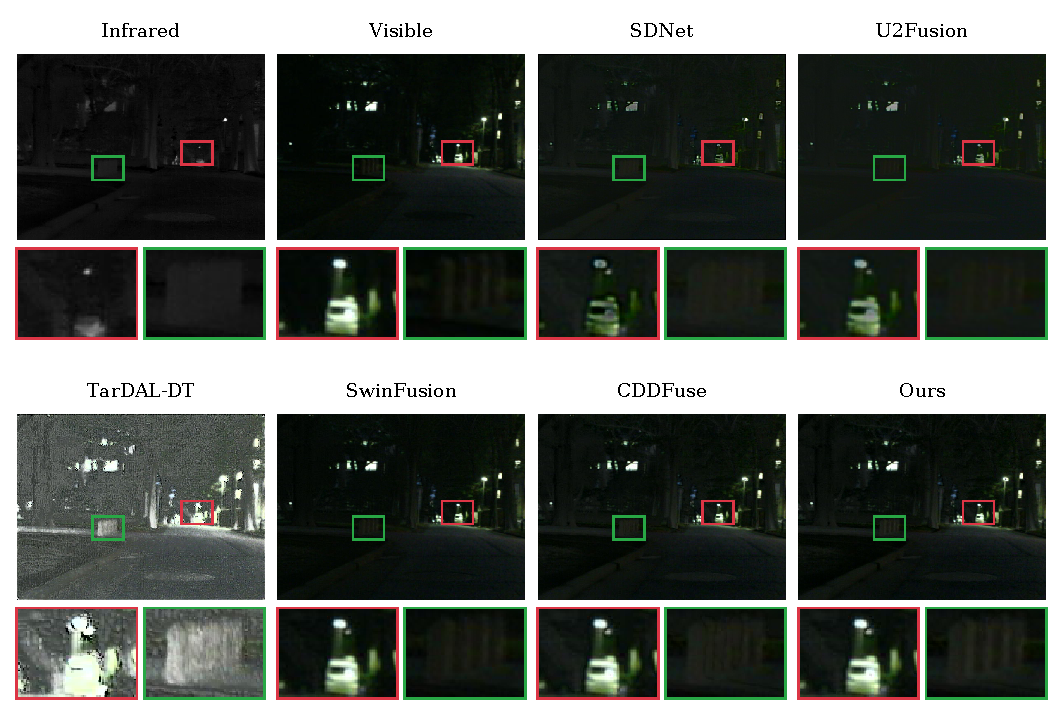
\includegraphics[width=0.98\textwidth]{figs/visual_sota_msrs.pdf}
\caption{Nighttime visual comparison. The red boxes enlarge a foreground target; the green boxes show background structures. Each full image is paired with the same two crops.}
\label{fig:visual_msrs}
\end{figure*}

\textbf{Daytime driving scene.}
\Cref{fig:visual_roadscene} contains a vehicle with different infrared and visible appearances, together with a bright building facade. SwinFusion's result has low contrast in the highlighted facade, making window and traffic-signal details less distinct. SCMFuse combines a visible rear-window boundary with thermal cues around the vehicle and retains the traffic signal and window outlines in the green crop. CDDFuse provides a similarly detailed result; the dataset-level VIF and $Q^{AB/F}$ improvements offer broader evidence for the proposed method than either selected image alone.

\begin{figure*}[!t]
\centering
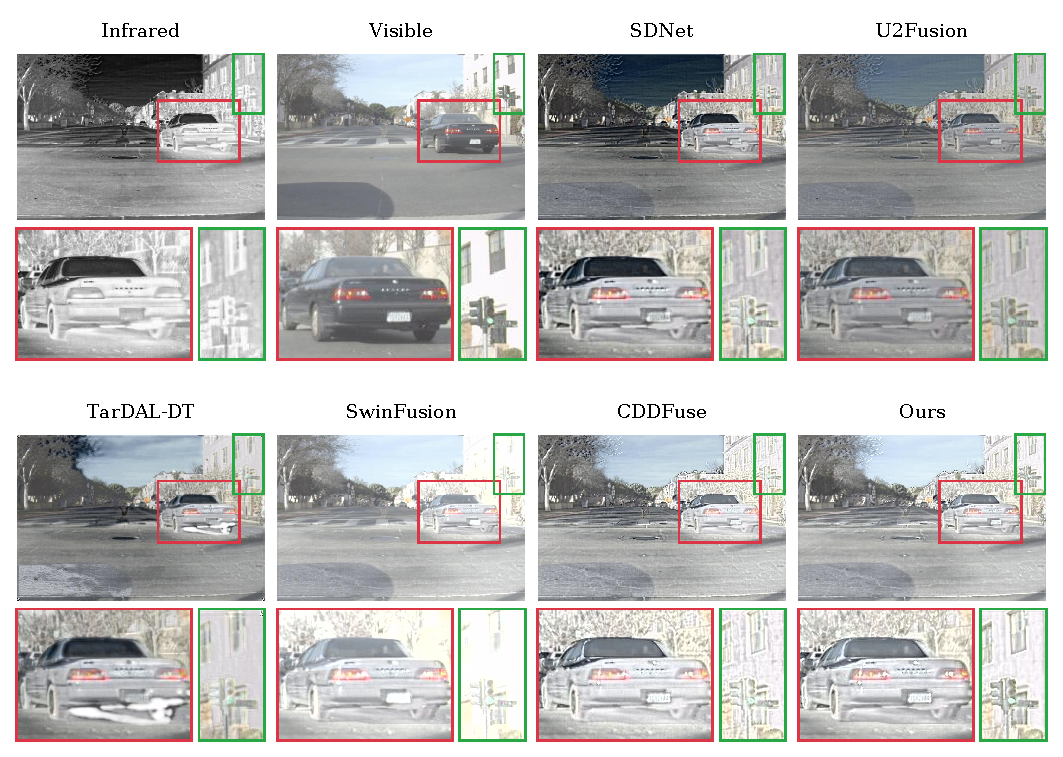
\includegraphics[width=0.98\textwidth]{figs/visual_sota_roadscene.pdf}
\caption{Daytime visual comparison. The red boxes highlight the vehicle, and the green boxes cover the traffic signal and building windows. Enlarged regions use the same locations across methods.}
\label{fig:visual_roadscene}
\end{figure*}
% Visual assets are retained without altering any fused result. Exact Ours checkpoint and TarDAL-DT/TarDAL mapping are recorded as provenance items in the final editorial review.

\subsection{Computational Efficiency}\label{subsec:efficiency}
\begin{table}[!t]
\centering
\caption{Reported model size and computational cost. Ours-P and Ours-C share the inference graph.}
\label{tab:complexity}
\small
\setlength{\tabcolsep}{8pt}
\begin{tabular}{@{}lrr@{}}
\toprule
Method & Params (M) & FLOPs (G)\\
\midrule
DenseFuse & 0.074 & 11.532\\
FusionGAN & 0.926 & 124.775\\
DIDFuse & 0.261 & 48.620\\
SDNet & 0.029 & 3.746\\
U2Fusion & 0.659 & 86.341\\
TarDAL & 0.297 & 38.768\\
SeAFusion & 0.167 & 21.758\\
SwinFusion & 0.974 & 149.365\\
FusionMamba & 164.539 & 92.076\\
CDDFuse & 1.188 & 235.716\\
Ours-P / Ours-C & 0.473 & 87.837\\
\bottomrule
\end{tabular}
\end{table}

\begin{table}[!t]
\centering
\caption{Training efficiency on the RTX 5070 Ti: 40 Phase I epochs and 80 Phase II epochs. Total time and speedup are rounded from the measured epoch durations.}
\label{tab:training}
\small
\setlength{\tabcolsep}{4pt}
\begin{tabular}{@{}lrrrr@{}}
\toprule
 & \multicolumn{2}{c}{Time (s/epoch)} & Total & Speedup\\
\cmidrule(lr){2-3}
Model & Phase I & Phase II & (h) & ($\times$)\\
\midrule
Baseline & 230.5 & 216.0 & 7.36 & 1.00\\
L (+SGC) & \textbf{126.4} & \textbf{111.7} & \textbf{3.89} & \textbf{1.89}\\
Ours-P & 138.1 & 135.6 & 4.55 & 1.62\\
Ours-C & 142.0 & 141.2 & 4.72 & 1.56\\
\bottomrule
\end{tabular}
\end{table}

\textbf{Model size and operations.}
As shown in \cref{tab:complexity}, SCMFuse uses $0.473$ M parameters and $87.837$ G FLOPs under the reported profile, compared with $1.188$ M and $235.716$ G for CDDFuse. The reductions are $60.2\%$ and $62.7\%$, respectively. Ours-P and Ours-C have identical model complexity because the additional supervision is evaluated only during training. Although several convolutional methods are smaller, SCMFuse combines its compact model with stronger fusion scores across multiple fidelity and structure metrics.
% Profiling input dimensions, operator coverage, and the specific baseline implementations were not independently remeasured; see final review.

The SGC and SCM Blocks contain point-wise projections with $\mathcal O(HWD^2)$ cost when kernel sizes, expansion ratios, state dimensions, and head counts are fixed. Both scale linearly with spatial size for fixed $D$. Pooling confines the four-directional scan to one-quarter of the original token count per direction for even image dimensions, while the main residual path remains full resolution. The resulting runtime benefit is evaluated through the measured latency rather than inferred from asymptotic complexity alone.

\textbf{Training and inference.}
\Cref{tab:training} shows that the lightweight configuration L reduces total training time from $7.36$ to $3.89$ hours. Ours-P and Ours-C require approximately $4.55$ and $4.72$ hours, corresponding to $1.62\times$ and $1.56\times$ acceleration. The contrast--structure terms add a small training overhead to the same inference architecture.

\begin{table*}[!t]
\centering
\caption{Inference latency (ms) and throughput (FPS) on the RTX 5070 Ti. Mean speedup is the arithmetic mean of the three dataset-specific latency ratios relative to CDDFuse. Best entries are bold.}
\label{tab:efficiency_comparison}
\small
\setlength{\tabcolsep}{9pt}
\begin{tabular}{@{}lrrrrrrr@{}}
\toprule
 & \multicolumn{2}{c}{MSRS} & \multicolumn{2}{c}{TNO} & \multicolumn{2}{c}{RoadScene} & Mean\\
\cmidrule(lr){2-3}\cmidrule(lr){4-5}\cmidrule(lr){6-7}
Model & ms & FPS & ms & FPS & ms & FPS & speedup\\
\midrule
SwinFusion & 412.5 & 2.42 & 1240.0 & 0.81 & 1385.2 & 0.72 & $0.80\times$\\
CDDFuse & 309.1 & 3.24 & 1017.3 & 0.98 & 1153.8 & 0.87 & $1.00\times$\\
L (+SGC) & \textbf{142.6} & \textbf{7.01} & 333.6 & 3.00 & 542.7 & 1.84 & $2.45\times$\\
Ours-P & 161.0 & 6.21 & \textbf{304.9} & \textbf{3.28} & \textbf{373.1} & \textbf{2.68} & $\mathbf{2.78\times}$\\
Ours-C & 160.6 & 6.23 & 310.4 & 3.22 & 373.9 & 2.67 & $2.76\times$\\
\bottomrule
\end{tabular}
\end{table*}

\Cref{tab:efficiency_comparison} reports inference time across the three datasets. Ours-C reduces MSRS latency from $309.1$ to $160.6$ ms, TNO latency from $1017.3$ to $310.4$ ms, and RoadScene latency from $1153.8$ to $373.9$ ms. Averaging these dataset-specific latency ratios gives a $2.76\times$ mean speedup. Ours-P achieves $2.78\times$. The two configurations share the same inference design; their small timing difference does not establish a runtime benefit from changing the loss. The efficiency gain is most pronounced on TNO and RoadScene, where the baseline has the largest latency.
% Timing precision, input resolutions, CUDA synchronization, I/O exclusion, warm-up and repetitions require the original benchmark script for full reproducibility.

\subsection{Ablation Studies}\label{subsec:ablation_study}
\textbf{Progressive configurations.}
\Cref{tab:main_ablation} evaluates four configurations: \textbf{B}, the CDDFuse baseline; \textbf{L}, B with the SGC-based encoder and hybrid decoder; \textbf{A}, L with the SCM Block, DGF, and MGF; and \textbf{F}, A with the proposed supervision. A and F correspond to Ours-P and Ours-C. Each step tests a defined set of changes within the complete framework.
% Historical mapping: B=Exp-0; L=Exp-1; A=manuscript Exp-2 / historical Exp-3_v2; F=manuscript Exp-3 / loss-enabled Exp-3_v2.
\begin{table*}[!t]
\centering
\caption{Progressive ablation. B: CDDFuse; L: lightweight encoder--decoder; A: L with the SCM Block, DGF, and MGF; F: A with the proposed supervision. A and F correspond to Ours-P and Ours-C. The best and second-best values are marked in \best{bold red} and \second{underlined blue}. Ties follow the displayed precision; all metrics are higher-is-better.}
\label{tab:main_ablation}
\small
\setlength{\tabcolsep}{7pt}
\begin{tabular}{@{}lrrrrrrrr@{}}
\toprule
Method & EN & SD & SF & MI & SCD & VIF & $Q^{AB/F}$ & SSIM\\
\midrule
\multicolumn{9}{c}{\textbf{MSRS}}\\
\midrule
B (Baseline) & 6.69 & 42.99 & \second{11.71} & \best{3.68} & 1.61 & \best{1.06} & \second{0.72} & \second{0.99}\\
L (+SGC) & \second{6.70} & \second{43.16} & 11.67 & \second{3.62} & \second{1.65} & \best{1.06} & \second{0.72} & \best{1.00}\\
A (+SCM and gates) & \second{6.70} & 43.02 & \best{11.75} & 3.35 & 1.61 & \best{1.06} & \best{0.73} & 0.98\\
F (+Supervision) & \best{6.73} & \best{43.31} & 11.66 & 3.45 & \best{1.70} & \best{1.06} & \best{0.73} & \second{0.99}\\
\midrule
\multicolumn{9}{c}{\textbf{TNO}}\\
\midrule
B (Baseline) & \second{7.10} & \second{45.47} & \second{13.49} & 2.41 & 1.64 & 0.79 & 0.56 & \second{0.98}\\
L (+SGC) & \best{7.11} & \best{45.73} & \best{13.50} & 2.35 & \best{1.72} & 0.81 & 0.56 & \best{1.01}\\
A (+SCM and gates) & 7.08 & 43.46 & 13.14 & \best{2.72} & 1.60 & \best{0.87} & \best{0.61} & 0.97\\
F (+Supervision) & 7.08 & 43.63 & 13.26 & \second{2.48} & \second{1.71} & \second{0.83} & \second{0.60} & \best{1.01}\\
\midrule
\multicolumn{9}{c}{\textbf{RoadScene}}\\
\midrule
B (Baseline) & 7.30 & 48.78 & \best{15.88} & 2.47 & 1.68 & 0.69 & 0.56 & \second{0.95}\\
L (+SGC) & \best{7.37} & \best{51.35} & 15.73 & 2.39 & \best{1.76} & 0.70 & 0.55 & \best{0.96}\\
A (+SCM and gates) & 7.30 & 49.17 & 15.71 & \best{2.62} & 1.62 & \best{0.77} & \best{0.62} & 0.92\\
F (+Supervision) & \second{7.32} & \second{50.12} & \second{15.84} & \second{2.54} & \second{1.72} & \second{0.75} & \second{0.61} & \second{0.95}\\
\bottomrule
\end{tabular}
\end{table*}


\textbf{Local processing (B $\to$ L).}
Replacing the shallow processing and decoder configuration increases throughput from $3.24$ to $7.01$ FPS on MSRS, $0.98$ to $3.00$ FPS on TNO, and $0.87$ to $1.84$ FPS on RoadScene. SD and SCD also increase on all three datasets, while VIF and $Q^{AB/F}$ remain close to the baseline. This establishes an efficient starting point for the deeper architectural changes.

\textbf{Space--channel modeling and fusion (L $\to$ A).}
The combined addition of the SCM Block and learned fusion gates improves TNO MI from $2.35$ to $2.72$, VIF from $0.81$ to $0.87$, and $Q^{AB/F}$ from $0.56$ to $0.61$. The corresponding RoadScene values increase from $2.39$, $0.70$, and $0.55$ to $2.62$, $0.77$, and $0.62$. MSRS $Q^{AB/F}$ rises to $0.73$. These results support the joint spatial--channel and aggregation design, particularly for transfer to the two other datasets.

\textbf{Proposed supervision (A $\to$ F).}
Adding the new objective raises SCD from $1.61/1.60/1.62$ to $1.70/1.71/1.72$ on MSRS/TNO/RoadScene. SD increases from $43.02/43.46/49.17$ to $43.31/43.63/50.12$, and SSIM from $0.98/0.97/0.92$ to $0.99/1.01/0.95$. MSRS MI also improves from $3.35$ to $3.45$. The full objective retains the MSRS VIF and $Q^{AB/F}$ values and trades a small portion of the TNO/RoadScene perceptual scores for higher structural correlation and contrast. The comparison evaluates the supervision package as a whole, rather than the contribution of each individual loss term.

\textbf{Intermediate architectural designs.}
\Cref{tab:mamba_variants} compares two exploratory designs with the final original-loss architecture. Variant V1 downsamples the base trunk and uses a scan-output channel normalization while retaining MDTA at the reduced resolution. Variant V2 uses channel scaling, removes MDTA, and applies an additional feature-rescaling operation. The final design retains the full-resolution residual stream and MDTA, and omits that feature rescaling.
\begin{table}[!t]
\centering
\caption{Intermediate base/fusion designs trained with the original objective. V1/V2 denote exploratory variants; Final is Ours-P. Best values are in bold.}
\label{tab:mamba_variants}
\small
\setlength{\tabcolsep}{4pt}
\begin{tabular}{@{}llrrrr@{}}
\toprule
Dataset & Variant & SD & MI & VIF & $Q^{AB/F}$\\
\midrule
MSRS & V1 & \textbf{43.15} & \textbf{3.45} & \textbf{1.06} & 0.72\\
 & V2 & 42.90 & 3.28 & \textbf{1.06} & \textbf{0.73}\\
 & Final & 43.02 & 3.35 & \textbf{1.06} & \textbf{0.73}\\
\midrule
TNO & V1 & \textbf{44.71} & 2.38 & 0.81 & 0.56\\
 & V2 & 44.22 & 2.53 & 0.83 & \textbf{0.61}\\
 & Final & 43.46 & \textbf{2.72} & \textbf{0.87} & \textbf{0.61}\\
\midrule
RoadScene & V1 & 48.51 & 2.50 & 0.72 & 0.58\\
 & V2 & \textbf{49.47} & 2.44 & 0.75 & 0.61\\
 & Final & 49.17 & \textbf{2.62} & \textbf{0.77} & \textbf{0.62}\\
\bottomrule
\end{tabular}
\end{table}

The final design achieves the highest TNO and RoadScene MI and VIF among these alternatives, with $Q^{AB/F}$ also leading or tying. Because several choices differ jointly, this comparison supports the integrated design rather than isolating normalization, resolution, or attention effects. Together with the progressive study, these results support the choice of the final architecture.
